\chapter{Tutorial: Processing Mars Orbiter Camera Imagery}
\label{ch:tutorial}

\section{Quick Start}

The programs in the Stereo Pipeline are command-line programs which
take a pair of images, and attempt to create a three-dimensional
point cloud from correlating them.  Then there are a few programs
that can convert that point cloud into a mesh for viewing or a
gridded terrain model for use in other ways.

So at the highest, most abstract level, if you have two image files
(say \texttt{image\_file1} and \texttt{image\_file2} ) this command
makes point clouds (and a bunch of other files):

\begin{verbatim}
    stereo image_file1 image_file2 stereo-output
\end{verbatim}
\noindent
Then you can make a mesh or a DEM file with either of the following
commands.  The \texttt{stereo-output-PC.tif} and
\texttt{stereo-output-L.tif} files are created by the \texttt{stereo}
program run above):

\begin{verbatim}
    point2mesh stereo-output-PC.tif stereo-output-L.tif

    point2dem stereo-output-PC.tif stereo-output-L.tif
\end{verbatim}
\noindent
There are a number of ways to fine-tune parameters and
analyze the results, but ultimately this software suite takes images
and builds models in a mostly automatic way.

% \section{Examples of Use}
%
% Download the tarball and it will unpack into a \texttt{p19} directory.  Create an output directory to hold the results, and invoke the \texttt{stereo} program:
%
% \begin{verbatim}
%       mkdir results
%       stereo E0201461.cub M0100115.cub results/p19
% \end{verbatim}
%
% You can look at the results by examining the disparity images. These
% show the horizontal and vertical components of the matching offsets
% for each pixel, and they can be a useful debugging tool if you want
% to check how the stereo matcher performed for a given stereo pair:
%
% \begin{verbatim}
%       cd results
%       disparitydebug p19-D.exr -o p19-D
%       disparitydebug p19-F.exr -o p19-F
% \end{verbatim}
%
% \emph{MJB: What exactly is being examined in the resultant images, what are users looking for?}
%
% A 3D mesh can be built from the point cloud and viewed using the
% \texttt{osgviewer} program:
%
% \begin{verbatim}
%       point2mesh p19-PC.tif p19-L.tif -o p19
%       osgviewer p19.ive
% \end{verbatim}
%
% When the \texttt{osgviewer} starts, you may want to turn off the
% lighting (hit the `L' key).
%
% A gridded DEM with floating point pixels can also be built from the point cloud:
%
% \begin{verbatim}
%       point2dem --xyz-to-lonlat -r mars p19-PC.tif -n -o p19
% \end{verbatim}
%
% You can also orthoproject the raw satellite imagery onto the DEM during this step:
%
% \begin{verbatim}
%       point2dem --xyz-to-lonlat -r mars p19-PC.tif -o p19 --orthoimage p19-L.tif
% \end{verbatim}
%
% Finally, you can create colorized, shaded relief (or both) images from the DEM, using these Vision Workbench programs:
%
% \begin{verbatim}
%       colormap p19-DEM.tif -o p19-colorized.tif
%       hillshade p19-DEM.tif -o p19-shaded.tif -e 25
%       colormap p19-DEM.tif --shaded-relief-file p19-shaded.tif -o p19-color-shaded.tif
% \end{verbatim}
%
% Finally, you can run the Vision Workbench's \texttt{image2qtree} on any of the following files:
%
% \begin{itemize}
% \item p19-DEM-normalized.tif
% \item p19-DRG.tif
% \item p19-shaded.tif
% \item p19-colorized.tif
% \item p19-shaded-colorized.tif
% \end{itemize}


\section{Preparing the Data}

The data set that is used in the tutorial and examples below is a pair
of Mars Orbiter Camera (MOC)
\citep{1992JGR....97.7699M,2001JGR...10623429M} images whose Planetary
Data System (PDS) Product IDs are M01/00115 and E02/01461.  These data
can be downloaded from the PDS directly, or they can be found in the
\texttt{data/MOC/} directory of your Stere Pipeline distribution.

These raw PDS images (\texttt{M0100115.imq} and \texttt{E0201461.imq})
need to be imported into the ISIS environment and radiometrically
calibrated.  You will need to be in an ISIS environment (have set the
\texttt{ISISROOT} environment variable and sourced the appropriate
ISIS 3 Startup script, as detailed in the ISIS 3 instructions, we will
denote this state with the `\texttt{ISIS 3>}' prompt).  Then you can
use the \texttt{mocproc} program.

\begin{verbatim}
    ISIS 3> mocproc from= M0100115.imq to= M0100115.cub Mapping= NO
\end{verbatim}
\noindent
There are also \texttt{Ingestion} and \texttt{Calibration} parameters
whose defaults are `\texttt{YES}' which will bring the image into
the ISIS format and perform radiometric calibration.  By setting
the \texttt{Mapping} parameter to `\texttt{NO}' the resultant file
will be an ISIS cube file that is calibrated, but not map-projected.
Note that while we have not explicitly run \texttt{spiceinit}, the
Ingestion portion of \texttt{mocproc} quietly ran \texttt{spiceinit}
for you (you'll find the record of it in the ISIS Session Log,
usually written out to a file named \texttt{print.prt}).

\begin{figure}[b!]
\begin{minipage}{5.2in}
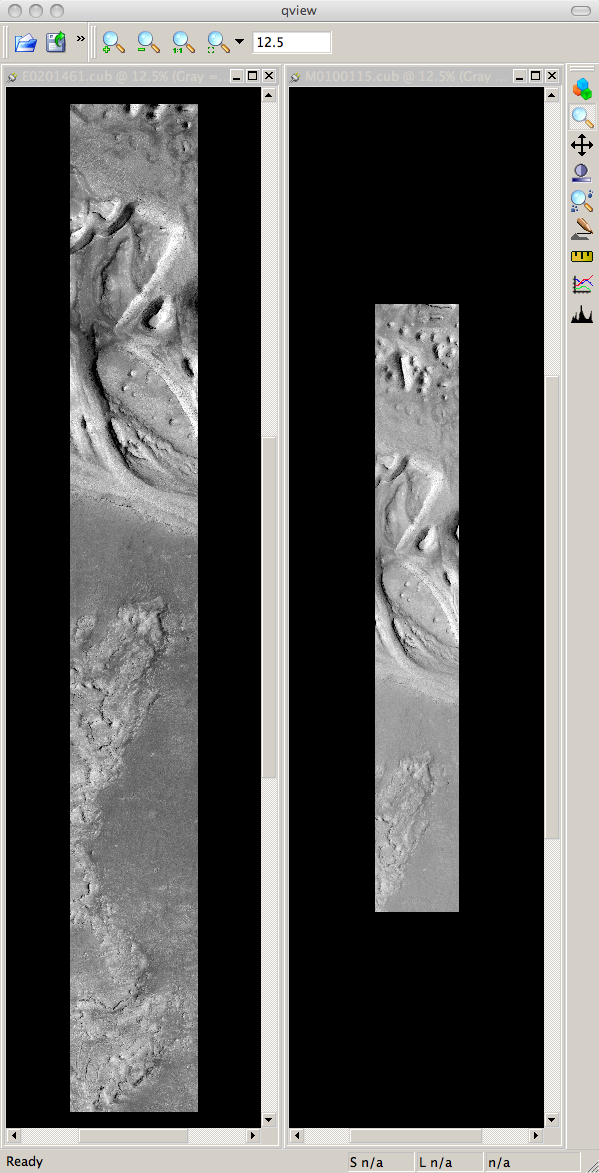
\includegraphics[height=3.7in]{images/p19-images.png}
\hfill
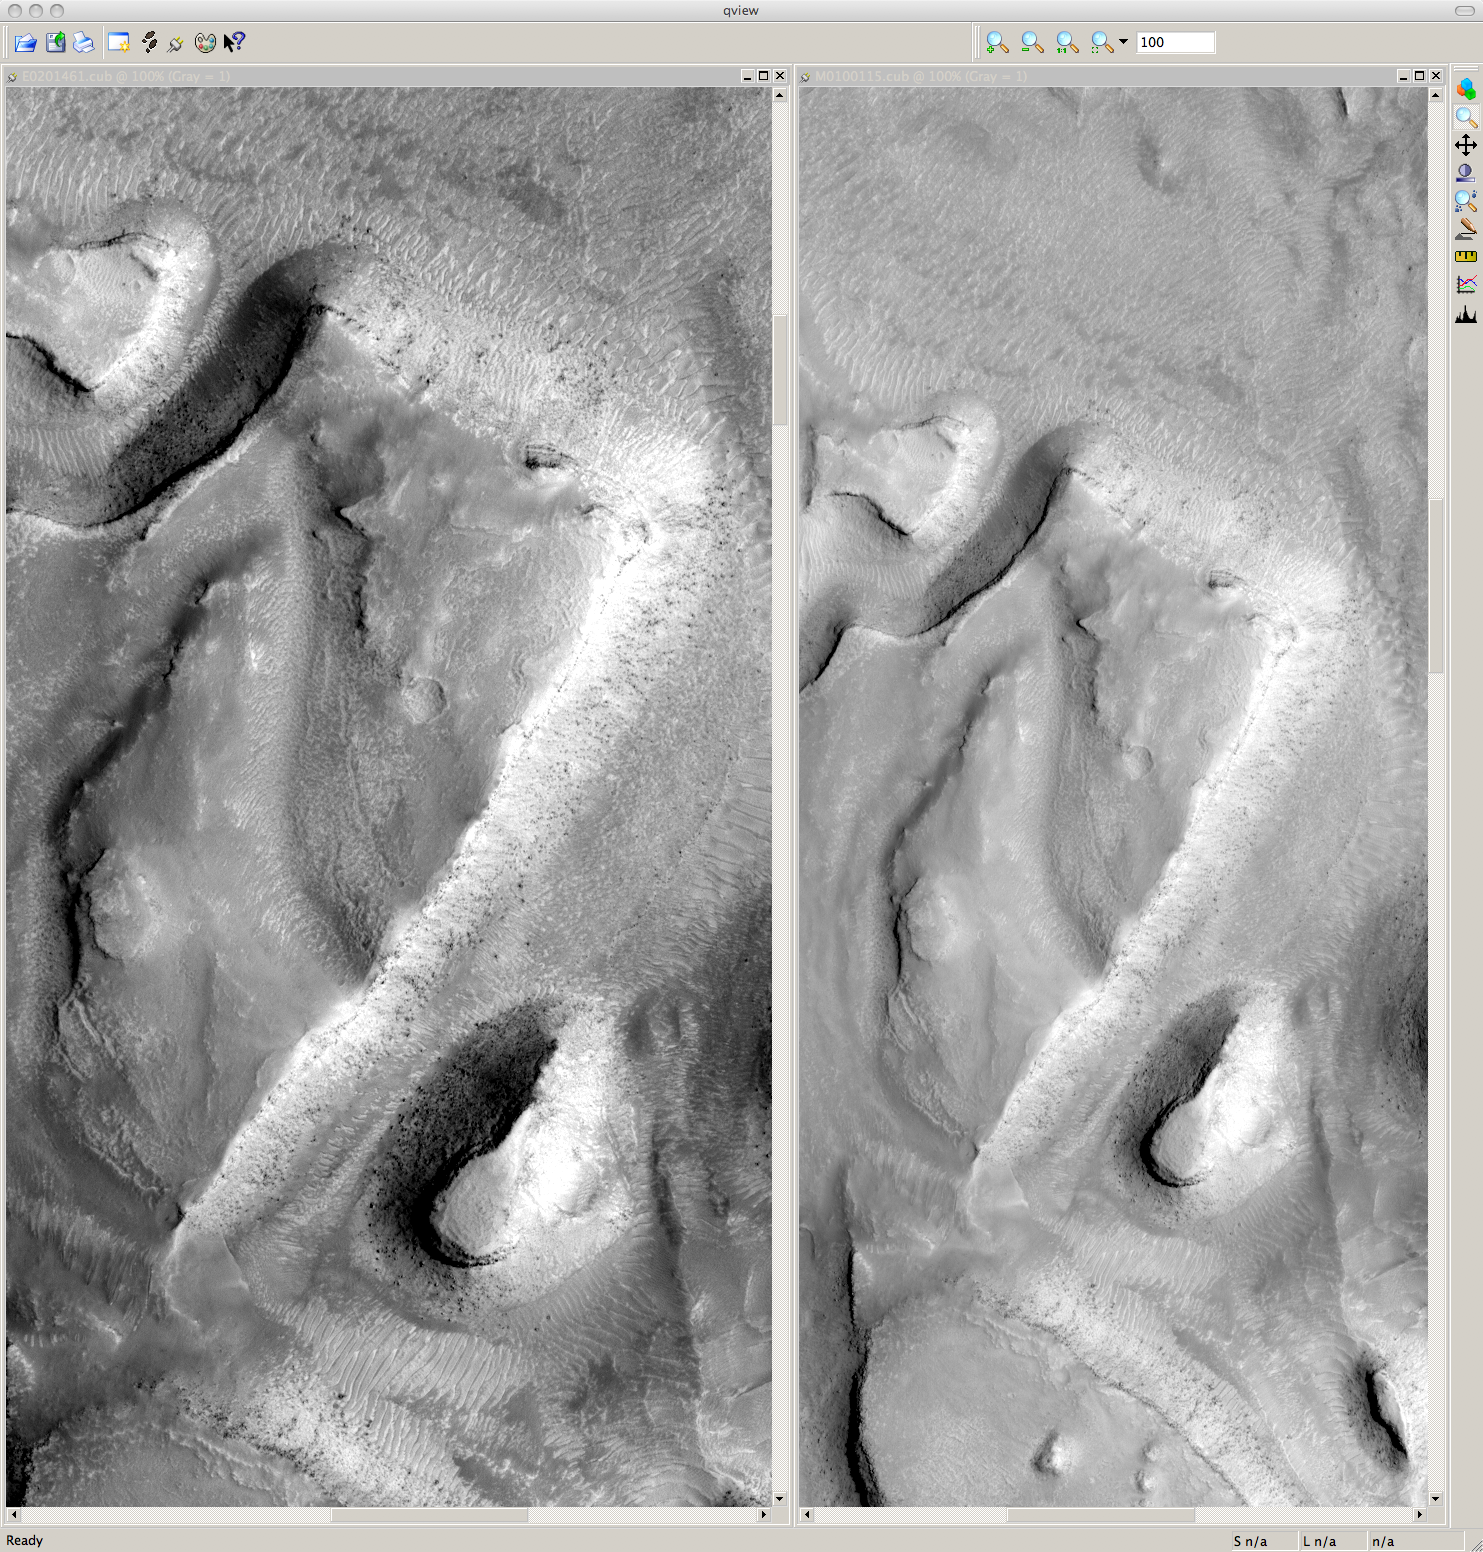
\includegraphics[height=3.7in]{images/p19-images_zoom.png}
\end{minipage}
\hfill
\begin{minipage}{1.3in}
\caption[P19 images open in qview zoomed in]{
    \label{p19-images}
    This figure shows \texttt{E0201461.cub} and \texttt{M0100115.cub}
    open in ISIS's qview program.  The view on the left shows their
    full extents at the same zoom level, showing how they have
    different ground scales.  The view on the right shows both images
    zoomed in on the same feature.  }
\end{minipage}
\end{figure}

\section{Running the Stereo Pipeline}

The following example will utilize images from the example MOC
dataset, discussed above.  The two example ISIS 3 image files are
\texttt{E0201461.cub} and \texttt{M0100115.cub}.

The \texttt{stereo} program (page \pageref{stereo}) is designed for
automated tie point matching and stereo production, and is the first
Stereo Pipeline tool we'll use.

If you like, you should create a directory for the results of the
processing.  The \texttt{stereo} program can generate a number of
output files, and we find it helpful to put them all in a directory,
but it isn't required.

\begin{verbatim}
    > ls
    E0201461.cub   M0100115.cub
    > mkdir results
\end{verbatim}
\noindent
The \texttt{stereo} program requires a \texttt{stereo.default} file
which can be altered for your needs.  Its contents are detailed on
page \pageref{ch:stereodefault}.  You may find it useful to save
multiple versions of the \texttt{stereo.default} file for various
processing needs. If you need to do that, be sure to specify which
configuration file \texttt{stereo} should use with the \texttt{-s}
option.  If this option is not given, the \texttt{stereo} program
will search for a file named \texttt{stereo.default} in the current
directory and will complain if there isn't one.

There is a \texttt{stereo.default} file included with the example
data set that is different from the example \texttt{stereo.default.example}
file distributed with the Stereo Pipeline.  The \texttt{stereo.default}
included with the example data set has a smaller correlation window
(smaller values for the \texttt{H\_CORR\_*} and \texttt{V\_CORR\_*}
variables) that is more suited to the MOC data.  You may want to
use both this \texttt{stereo.default} and the
\texttt{stereo.default.example} to explore how the results are
different.

Alternatively, it is possible to not have to define the
\texttt{H\_CORR\_*} and \texttt{V\_CORR\_*} in
\texttt{stereo.default}. When this happens, \texttt{stereo} will
collect interest points on a reduced version of the input images to
guess the correct search range. Afterwards, \texttt{stereo} prints its
estimation of a search window in the terminal. This guess for a search
window can be used as a starting point for a better search range if
the results for the first time are unacceptable.

Here is how the \texttt{stereo} program is called (there should be a
\texttt{stereo.default} file distributed along with the example data
set that will be used):

\begin{verbatim}
    ISIS 3> stereo E0201461.cub M0100115.cub results/E0201461-M0100115
\end{verbatim}

\noindent
That last option (\emph{results/E0201461-M0100115}) can be anything you
want it to be.  It designates the text that \texttt{stereo} will use
as a prefix for its many output files.  Since the first part is
\texttt{results/} this causes the program to put the results in that
directory with files whose names start with
\texttt{E0201461-M0100115}. If instead that last text was just
\texttt{E0201461-M0100115} it would have created a bunch of files that
start with \texttt{E0201461-M0100115} in the same directory as the
input files.

The \texttt{stereo} program's processing moves through several
stages which are detailed on page \pageref{entrypoints}.  However,
once the \texttt{stereo} program completes, it creates a number of
files.  A quick look at some of the TIFF files created, can quickly
give you an idea of what the \texttt{stereo} program did (figure
\ref{p19-stereo-output}).

\begin{figure}
\begin{center}
\includegraphics[width=5in]{images/p19-stereo-output.png}
\caption[P19 stereo output images]{
    \label{p19-stereo-output}
	These are the four viewable \texttt{.tif} files created by
	the \texttt{stereo} program.  The left two are the aligned
	images (\texttt{E0201461-M0100115-L.tif} and
	\texttt{E0201461-M0100115-R.tif}).  The next two images are
	the mask images (\texttt{E0201461-M0100115-lMask.tif} and
	\texttt{E0201461-M0100115-rMask.tif}), which indicate which
	pixels in the aligned images are good to use for the next
	step.  The image on the right is the Good Pixel map
	(\texttt{E0201461-M0100115-GoodPixelMap.tif}), which indicates
	the pixels in grey which were successfully matched with the
	correlator.  The red pixels were not.  Those red pixels which
	are not black in both mask images are optionally filled later
	during the hole-filling step.
    }
\end{center}
\end{figure}

% \begin{figure}
% \begin{center}
% 
\includegraphics[height=8in]{images/p19-goodpixel.png}
% \caption[P19 good pixel image]{
%     \label{p19-goodpixel}
% 	The Good Pixel map.
% 	Red pixels are not useful for alignment.
%     }
% \end{center}
% \end{figure}
%
% \begin{figure}
% \begin{center}
% 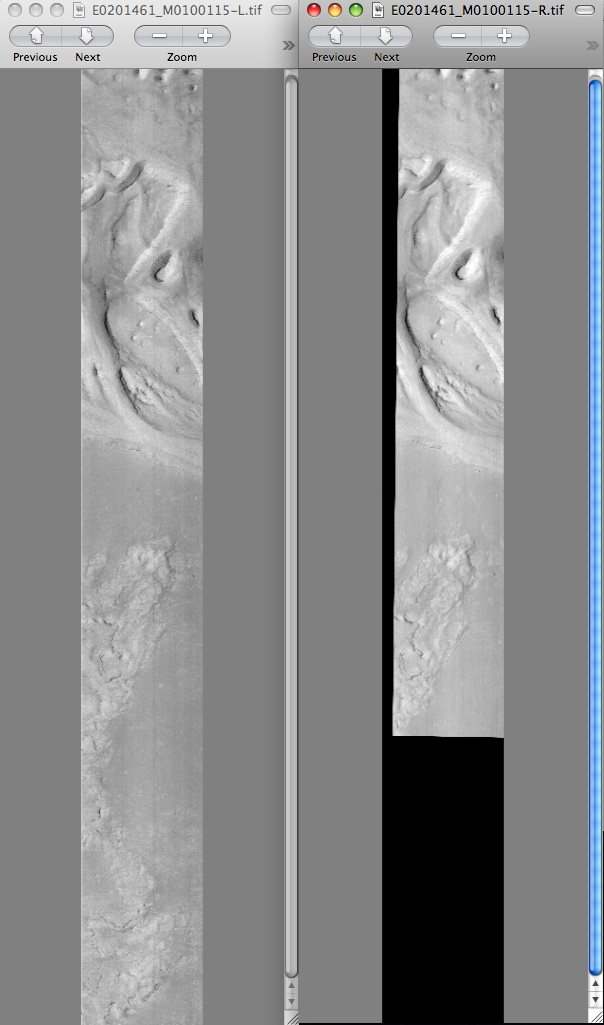
\includegraphics[width=3in]{images/p19-aligned.png}
% \caption[P19 aligned image]{
%     \label{p19-aligned}
% 	The left and right aligned images.
%     }
% \end{center}
% \end{figure}

If those TIFF files look okay, you can probably just go on to making
a mesh or a DTM from the point cloud file
(\texttt{E0201461-M0100115-PC.tif}).  The most important file is
the Good Pixel Map (\texttt{E0201461-M0100115-GoodPixelMap.tif}).
If this file shows mostly good, gray pixels in the overlap area
(the area that is white in both the \texttt{E0201461-M0100115-lMask.tif}
and \texttt{E0201461-M0100115-rMask.tif} files), then you're probably
good to go.  If this shows bad, red pixels in the overlap area,
then you'll probabaly need to go back and tune your \texttt{stereo.default}
file.  The example data also contains a \texttt{stereo.bad} file
which has intentionally bogus values for the dimensions of the
correlation window.  You can run \texttt{stereo} with the \texttt{-s
stereo.bad} command to see what the Good Pixel Map looks like with
this.

To get an idea of the disparity information that the \texttt{stereo}
program created and then used to build the point cloud, it can be
useful to take a look at that disparity information.  The \texttt{stereo}
program records this information in several \texttt{.exr} disparity
files.

To get a look at the disparity information, you need to convert it
into a more viewable format.  Move into the directory that contains
your results, and run the \texttt{disparitydebug} program (page
\pageref{disparitydebug}) to create the the horizontal and vertical
components of the disparity (matching offsets for each pixel).

\begin{figure}[b!]
\begin{minipage}{4in}
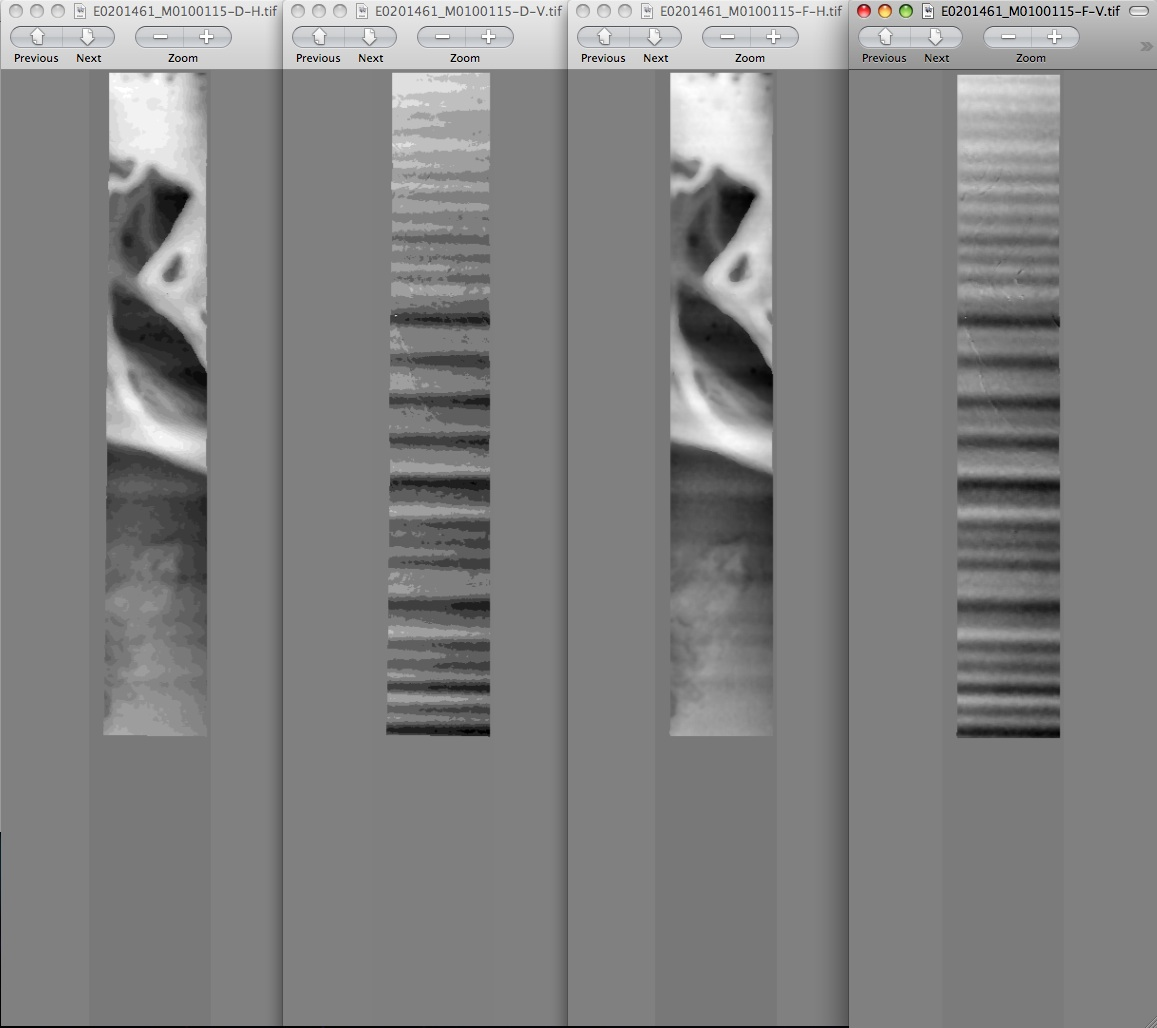
\includegraphics[width=4in]{images/p19-disparity.png}
\end{minipage}
\hfill
\begin{minipage}{2.7in}
\caption[P19 disparity images]{
    \label{p19-disparity}
	The disparity images.  The two images on the left are the
	\texttt{E0201461-M0100115-D-H.tif} and
	\texttt{E0201461-M0100115-D-V.tif} files, which are the raw horizontal and
	vertical disparity components.  The two images on the right are the
	\texttt{E0201461-M0100115-F-H.tif} and
	\texttt{E0201461-M0100115-F-V.tif} files, which are the final
	filtered, sub-pixel disparity map with outlier removal and holes
	filled in, and is what will be used to build the point cloud.  Since
	these MOC images were acquired by rolling the spacecraft across-track,
	most of the disparity that represents topography is present in the
	horizontal disparity map.  The vertical disparity map shows disparity
	not from topography, but from spacecraft movement.
    }
\end{minipage}
\end{figure}

\begin{verbatim}
    cd results
    disparitydebug E0201461-M0100115-F.exr
\end{verbatim}

\noindent
The two output files, \texttt{E0201461-M0100115-F-H.tif} and
\texttt{E0201461-M0100115-F-V.tif} are normalized images of the
horizontal (H) and vertical (V) disparity.  `Normalized' is a key
word here.  You can see that the horizontal and vertical disparity
images in figure \ref{p19-disparity} have the same range of gray
values from white to black, but they represent significantly different
absolute amounts of disparity.  These files are useful if you want
to check the performance of the \texttt{stereo} program for any
given stereo pair.

There are actually four flavors of disparity map: the \texttt{-D.exr},
the \texttt{-R.exr}, the \texttt{-F-corrected.exr}, and \texttt{-F.exr}.
You can run \texttt{disparitydebug} on any of them, and actually taking a
look at all of them can show you the differences between the disparity maps
at the different stages of processing.

\section{Visualizing the Results}

When \texttt{stereo} finishes up, it will have produced a point cloud.
At this point, the processing fans out, as many kinds of data
products can be built from the \texttt{E0201461-M0100115-PC.tif}.

One of the things that can be done is to produce a 3D mesh with
\texttt{point2mesh} (page \pageref{point2mesh}). This is not a science
product, but is just a quick visualization that can show the data
rendered in 3D. The mesh produced can be viewed with
\texttt{osgviewer} (the Open Scene Graph Viewer program, distributed
with the binary version of the Stereo Pipeline).  The
\texttt{point2mesh} program takes the point cloud file and the left
normalized image created by \texttt{stereo} as inputs.

\begin{verbatim}
    point2mesh E0201461-M0100115-PC.tif E0201461-M0100115-L.tif -l
\end{verbatim}

\noindent
This will create the file \texttt{E0201461-M0100115.ive}, openable
with \texttt{osgviewer}. When the \texttt{osgviewer} program starts,
you may want to turn off the lighting (hit the `L' key).

\begin{figure}[h]
\begin{minipage}{5in}
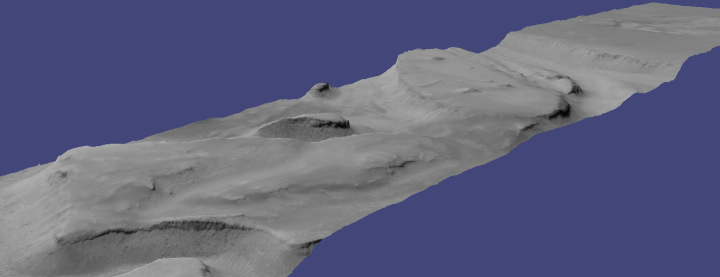
\includegraphics[width=5in]{images/p19-osg.png}
\end{minipage}
\hfill
\begin{minipage}{1.7in}
\caption[P19 in OSG]{
    \label{p19-osg}
	This shows the \texttt{E0201461-M0100115.ive} file displayed in
	the OSG Viewer.
    }
\end{minipage}
\end{figure}

The \texttt{point2dem} program (page \pageref{point2dem}) creates
a digital elevation model (DEM) from the Point Cloud file.

\begin{verbatim}
    point2dem E0201461-M0100115-PC.tif
\end{verbatim}

The resultant file, \texttt{E0201461-M0100115-DEM.tif}, will have
32-bit pixels, and so (much like the \texttt{E0201461-M0100115-PC.tif}
file) will not render well in typical image viewers. The resulting TIF
file is also contain georeferencing information which is useful for
working with other GIS platforms.

You can specify a coordinate system (e.g., latlon) and a reference
spheroid (i.e., calculated for the Moon or Mars). You also have the
option of creating a normalized DEM in addition to the automatically
generated non-normalized DEM. The normalized DEM again is just for
visualization and checking the quality of the product.

\begin{verbatim}
    point2dem --xyz-to-lonlat -r mars -n E0201461-M0100115-PC.tif
\end{verbatim}

\noindent
The \texttt{point2dem} program can also be used to orthoproject raw
satellite imagery onto the DEM. To do this, invoke \texttt{point2dem}
just as before, but add the \texttt{orthoimage} option and specify
the use of the left image file as the texture file to use for the
projection

\begin{verbatim}
    point2dem --xyz-to-lonlat -r mars --orthoimage E0201461-M0100115-L.tif \
      E0201461-M0100115-PC.tif
\end{verbatim}

\noindent
The \texttt{point2dem} program can be used in many different ways.
Be sure to explore all of the options.

\begin{figure}
\begin{minipage}{4in}
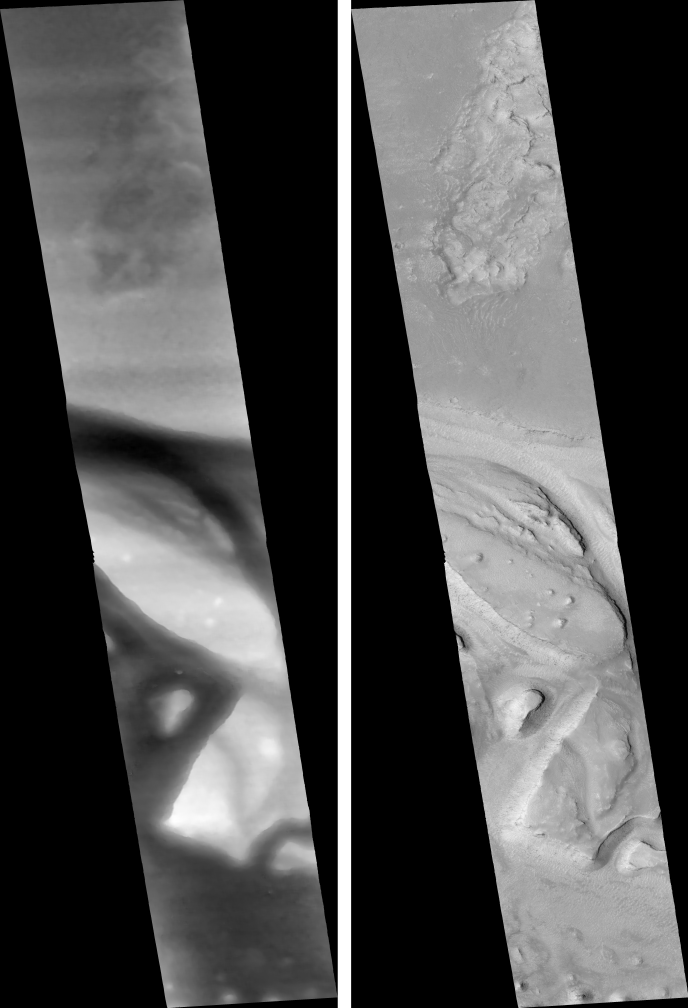
\includegraphics[width=4in]{images/p19-norm_ortho.png}
\end{minipage}
\hfill
\begin{minipage}{2.7in}
\caption[P19 Normalized DEM and Orthophoto]{
    \label{p19-norm_ortho}
	The image on the left is a normalized DEM (using the
	\texttt{-n} option) which which shows low terrain values
	as black and high terrain values as white (in a 0 to 255
	sense).  The image on the right is the orthographic image
	(created using the \texttt{--orthoimage} option to
	\texttt{point2dem}).
    }
\end{minipage} \end{figure}

% \begin{figure}
% \begin{center}
% 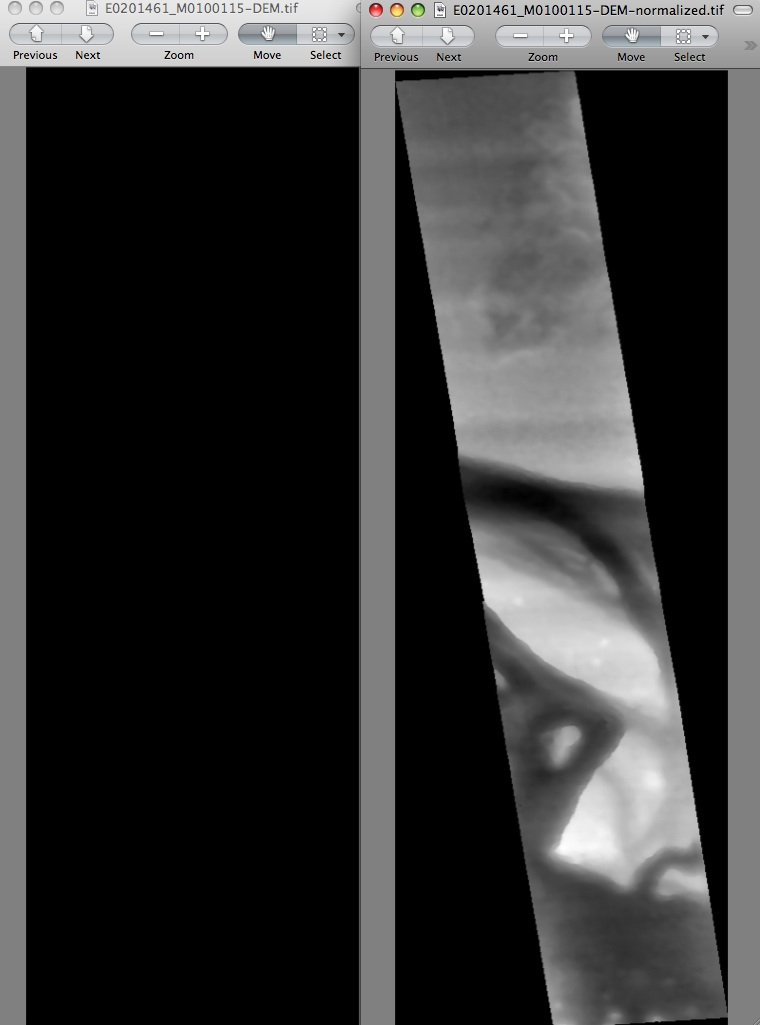
\includegraphics[width=4in]{images/p19-dems.png}
% \caption[P19 dem images]{
%     \label{p19-dems}
% 	The non-normalized and normalized DEMs. Note that the
% 	non-normalized version contains floating point pixel values
% 	and will not open in most image viewing programs which
% 	expect integer pixel values between 0 and 255 (which is
% 	what the normalized version does for you).
%     }
% \end{center}
% \end{figure}
%
% \begin{figure}
% \begin{center}
% \includegraphics[width=3in]{images/p19-ortho.png}
% \caption[P19 orthophoto]{
%     \label{p19-ortho}
% 	The left image orthoprojected onto the DEM.
%     }
% \end{center}
% \end{figure}

Once you have generated a DEM file, you can use the Vision Workbench's
\texttt{colormap} and \texttt{hillshade} tools to create colorized
and/or shaded relief images from the DEM.

To create a colorized version of the DEM, you need only specify the
DEM file to use. Yet alternatively you can specific your own min and
max color ranges.

\begin{verbatim}
    colormap p19-DEM.tif -o p19-colorized.tif
\end{verbatim}

To create a hillshade of the DEM, you should specify the DEM file
to use. It is also advisable to explore the effects of altering the
elevation of the light source.

\begin{verbatim}
    hillshade p19-DEM.tif -o p19-shaded.tif -e 25
\end{verbatim}

To create a colorized version of the shaded relief file, specify
the DEM and the shaded relief file that should be used.

\begin{verbatim}
    colormap p19-DEM.tif --shaded-relief-file p19-shaded.tif -o p19-color-shaded.tif
\end{verbatim}

\begin{figure}
\begin{center}
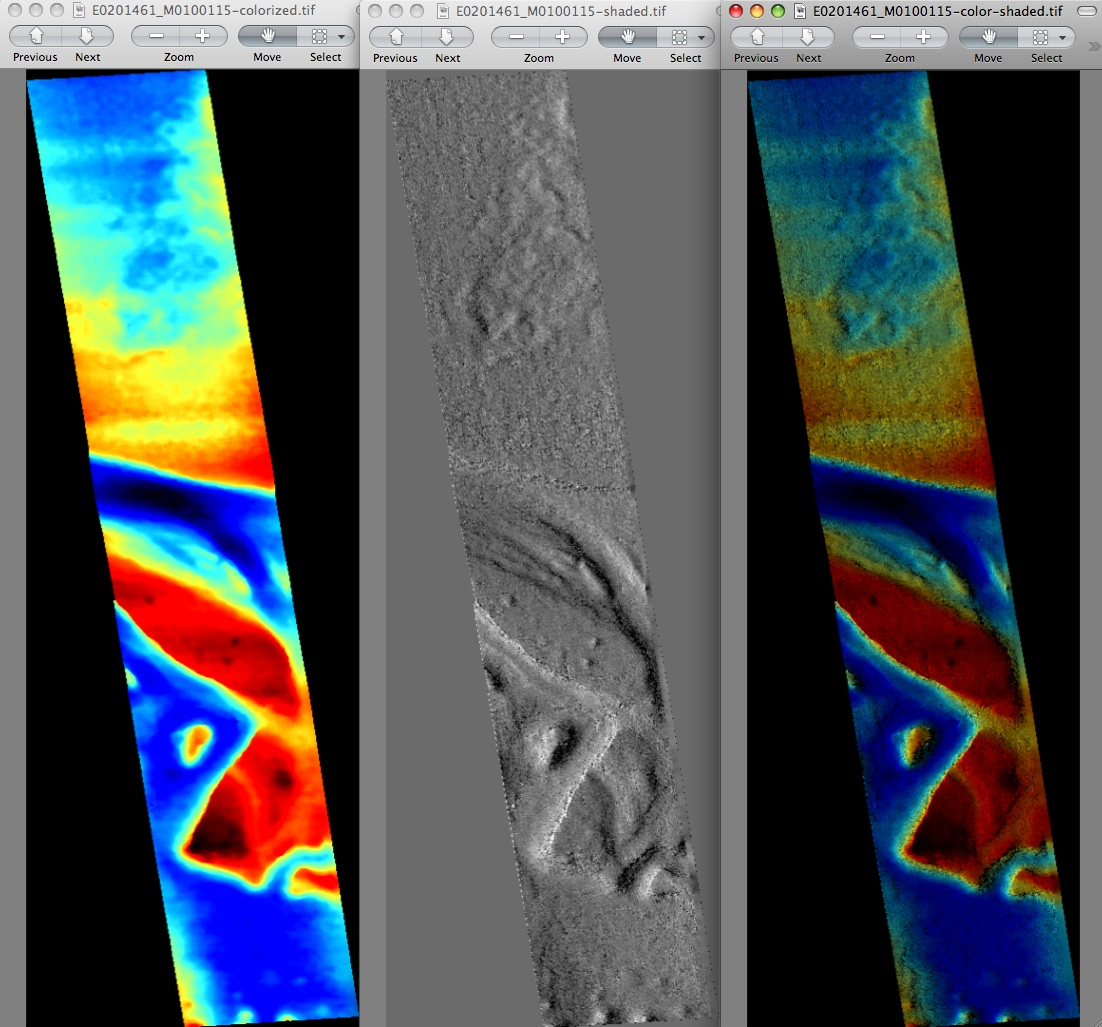
\includegraphics[width=5in]{images/p19-colorized-shaded.png}
\caption[P19 colorized and shaded relief]{
    \label{p19-color}
	The colorized DEM, the shaded relief image, and the colorized hillshade.
    }
\end{center}
\end{figure}

The final option of the stereo processing package is
\texttt{image2qtree}.  This function was designed for use in creating
geographically referenced images in tiles such that each tile can be
viewed at ideal resolution. It can also be used to create KML files
that can be viewed in Google Earth. The program can be used on any of
the following files that you have generated:
\begin{verbatim}
    p19-DEM-normalized.tif
    p19-DRG.tif
    p19-shaded.tif
    p19-colorized.tif
    p19-shaded-colorized.tif
\end{verbatim}

Specify which image you would like to invoke \texttt{image2qtree}
on. Below makes an overlay that can be viewed in Google Mars.

\begin{verbatim}
    image2qtree p19-DEM-normalized.tif -m kml --draw-order 100
\end{verbatim}


%% \section{Preparing Selected Data}

%% There are many ways to process different kinds of image data, and
%% some will be more appropriate for operations by the Stereo Pipeline
%% than others.  While we strive to make the Stereo Pipeline extensible
%% and robust, there are a limited (but growing) set of data that we
%% have thoroughly tested.

%% This section outlines the suggested pre-processing steps to prepare
%% specific data sets for use in the Stereo Pipeline.

%% \subsection{Mars Oribiter Camera (MOC)}

%% MOC images (ending in \texttt{.imq} or \texttt{.img}) can be downloaded from
%% the PDS and only require a single ISIS command to prepare for Stereo Pipeline use:

%% \begin{verbatim}
%%     ISIS 3> mocproc from= MOCimage.imq to= MOCimage.cub Mapping= NO
%% \end{verbatim}

%% The resulting ISIS cube file (e.g. \texttt{MOCimage.cub}) is now ready
%% for processing by the \texttt{stereo} program.


%% \subsection{High Resolution Imaging Science Experiment (HiRISE)}

%% HiRISE images are more complicated.

%% At the moment, the `best' processing method is to start with HiRISE
%% \texttt{*.balance.cub} files (available only internally to the
%% HiRISE team) and run them through the USGS's \texttt{hinoproj.pl}
%% script.  This results in \texttt{noproj}ed and de-jittered cube
%% files that can be run.

%% In the future (who knows when), the HiRISE team will directly produce
%% \texttt{noproj}ed images (dejittered through a different, improved,
%% algorithm) which will be available in the \texttt{extras/} directory
%% of the HiRISE PDS Volume.  And those images will probably be directly
%% usable by the Stereo Pipeline.

%% \emph{As you can tell, I'm still in the process of tracking all of this down. -RAB}
